\documentclass{article}

\usepackage{graphicx}
\usepackage{tikz}
\usepackage{tikzsymbols}
\usetikzlibrary{calc,patterns,shapes.geometric}
\pagestyle{empty}
\usepackage[margin=0pt]{geometry}
\geometry{papersize={14in,12in}}

\def\centerarc[#1](#2)(#3:#4:#5){\draw[#1] ($(#2)+({#5*cos(#3)},{#5*sin(#3)})$) arc (#3:#4:#5);}

\begin{document}
	\begin{figure}
		\centering
		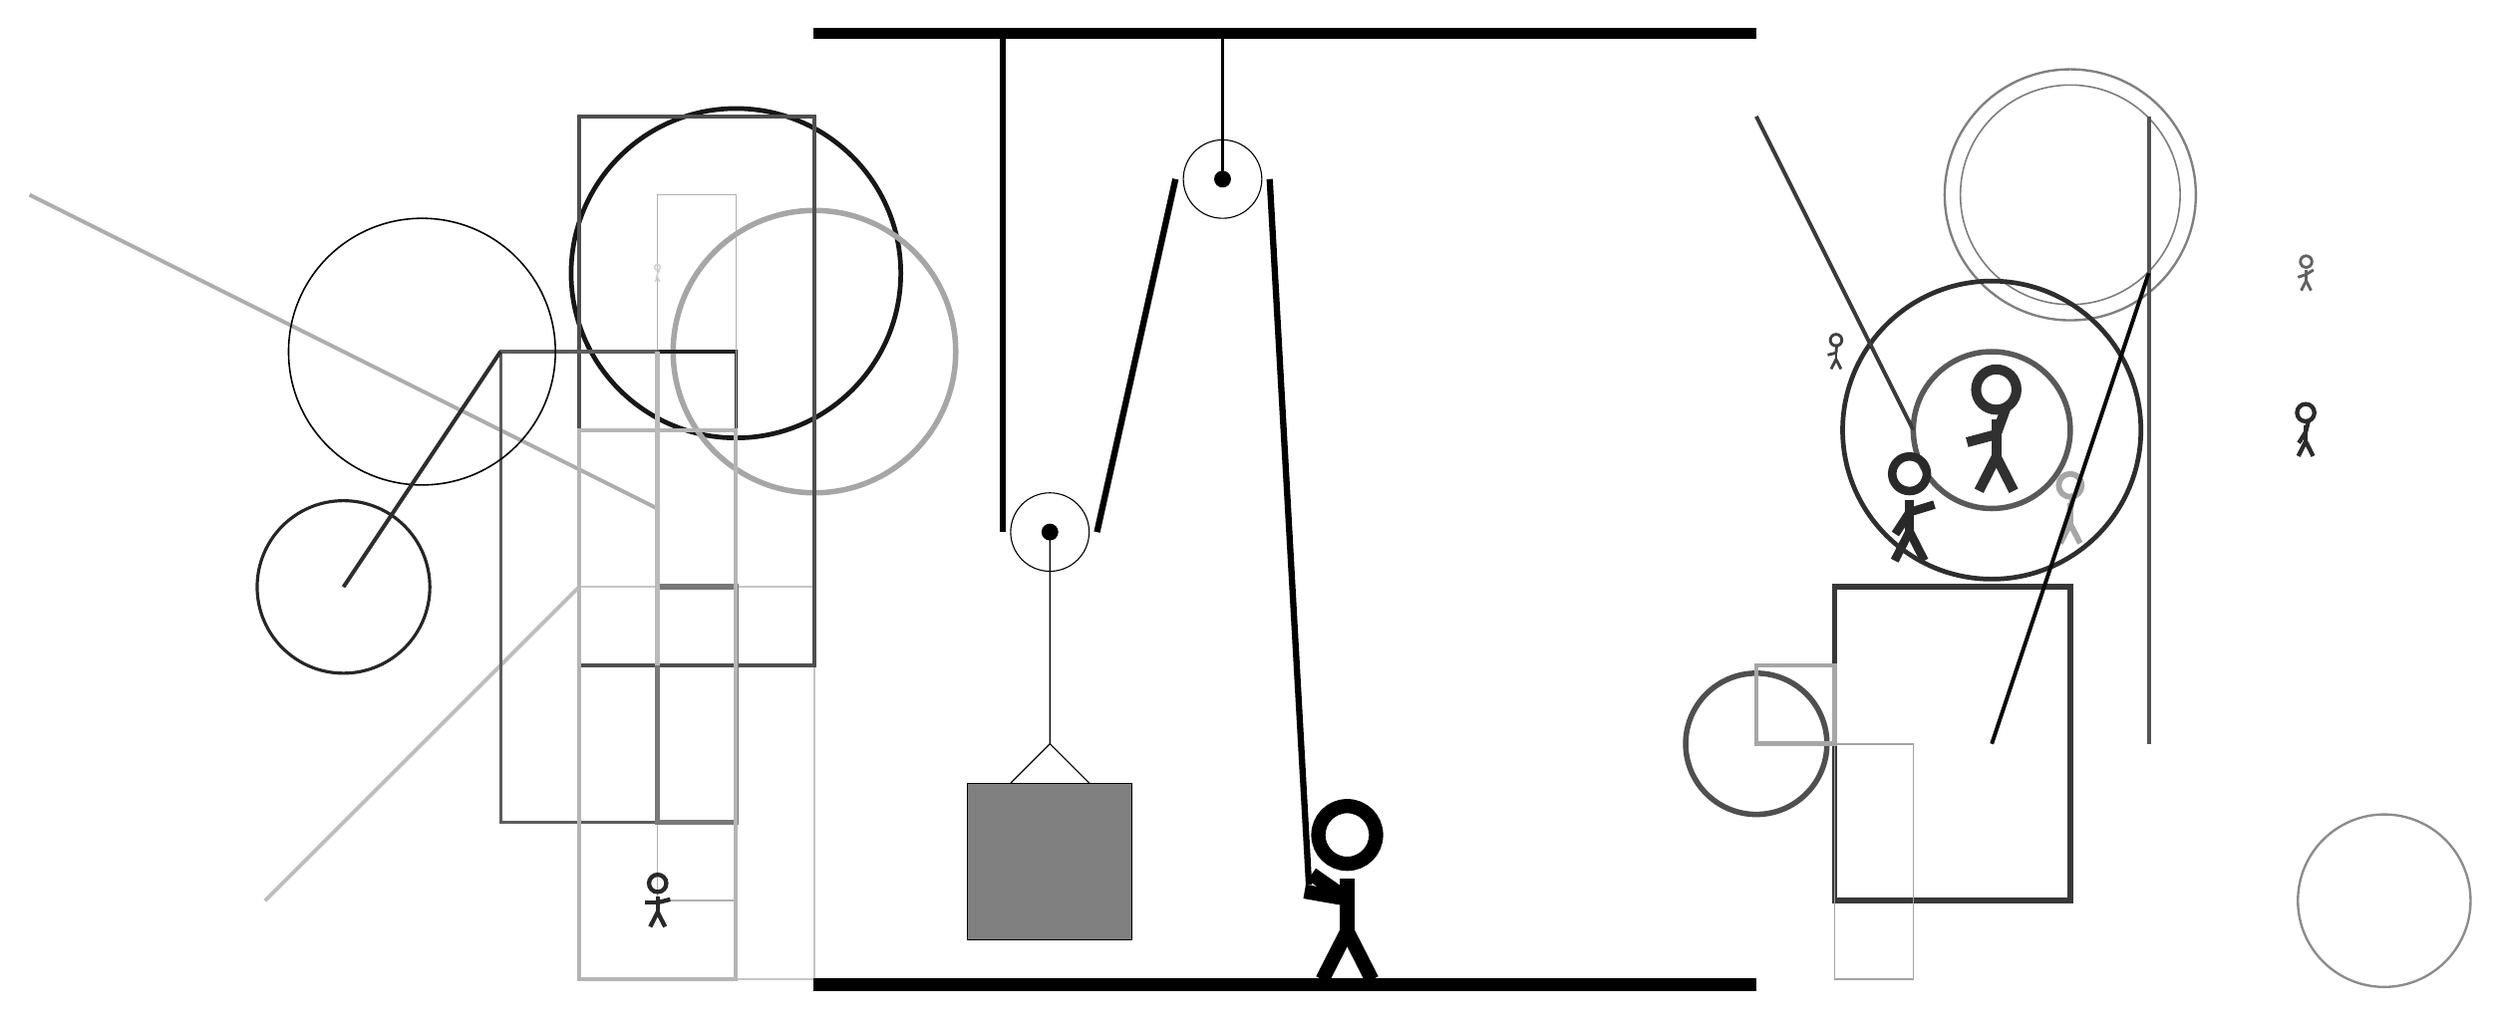
\begin{tikzpicture}
			%%%%% START %%%%%
			
			\draw[fill=black] (-2, 9) rectangle (10, 9.125);
			
			\draw (3.2, 7.2) circle (0.5);
			\draw[fill=black] (3.2, 7.2) circle (0.1);
			\draw[thick] (3.2, 7.2) -- (3.2, 9);
			
			\draw[line width=0.5mm, color=black!26](-5, 2) -- (-9, -2);
			
			\draw[line width=0.3mm, color=black!22] (-2, 2) rectangle (-5, -3);
			\draw [line width=0.3mm, color=black!50](14, 7) circle (1.6);
			\draw [line width=0.6mm, color=black!91](-3, 6) circle (2.1);
			
			\draw [line width=0.7mm, color=black!35](-2, 5) circle (1.8);
			\draw[line width=0.4mm, color=black!87] (-3, 5) rectangle (-5, 1);
			\draw [line width=0.3mm, color=black!45](18, -2) circle (1.1);
			\draw[line width=0.2mm, color=black!31] (-3, 7) rectangle (-4, -2);
			\node[line width=0.7mm, color=black!75] at (11, 5) {\Strichmaxerl[2][14][86]};
			
			\draw[line width=0.5mm, color=black!32](-4, 3) -- (-12, 7);
			\node[line width=0.4mm, color=black!84] at (-4, -2) {\Strichmaxerl[3][0][14]};
			\draw [line width=0.7mm, color=black!65](13, 4) circle (1.0);
			\node[line width=0.6mm, color=black!62] at (17, 6) {\Strichmaxerl[2][19][32]};
			\node[line width=0.2mm, color=black!84] at (12, 3) {\Strichmaxerl[6][57][17]};
			\draw[line width=0.5mm, color=black!69] (-2, 1) rectangle (-5, 8);
			\node[line width=0.4mm, color=black!35] at (14, 3) {\Strichmaxerl[4][82][80]};
			\draw [line width=0.2mm, color=black!51](14, 7) circle (1.4);
			\node[line width=0.3mm, color=black!81] at (13, 4) {\Strichmaxerl[7][15][70]};
			\draw [line width=0.4mm, color=black!85](-8, 2) circle (1.1);
			\draw[line width=0.7mm, color=black!78] (11, 2) rectangle (14, -2);
			\draw [line width=0.6mm, color=black!82](13, 4) circle (1.9);
			
			\draw[line width=0.5mm, color=black!67](15, 8) -- (15, 0);
			
			\draw[line width=0.5mm, color=black!97](13, 0) -- (15, 6);
			\node[line width=0.7mm, color=black!19] at (-4, 6) {\Strichmaxerl[1][72][61]};
			\draw[line width=0.4mm, color=black!64] (-4, 5) rectangle (-6, -1);
			\draw [line width=0.7mm, color=black!69](10, 0) circle (0.9);
			\draw[line width=0.6mm, color=black!35] (10, 1) rectangle (11, 0);
			\draw[line width=0.2mm, color=black!36] (11, 0) rectangle (12, -3);
			\draw [line width=0.2mm, color=black!100](-7, 5) circle (1.7);
			\draw[line width=0.5mm, color=black!82](-6, 5) -- (-8, 2);
			\draw[line width=0.7mm, color=black!53] (-3, -1) rectangle (-4, 2);
			
			\draw[line width=0.5mm, color=black!29] (-3, 4) rectangle (-5, -3);
			\draw[line width=0.5mm, color=black!77](12, 4) -- (10, 8);
			\node[line width=0.7mm, color=black!83] at (17, 4) {\Strichmaxerl[3][58][76]};
			\draw[line width=0.6mm, color=black!27] (-4, 5) rectangle (-4, 1);
			
			\draw (1, 2.7) circle (0.5);
			\draw[fill=black] (1, 2.7) circle (0.1);
			
			\draw (1, 2.7) -- (1, 0) -- (0.5, -0.5);
			\draw (1, 0) -- (1.5, -0.5);
			\draw[fill=black!50] (-0.05, -0.5) rectangle (2.05, -2.5);
			
			\draw[line width=0.8mm] (0.4, 9) -- (0.4, 2.7);
			\centerarc[line width=0.8mm](1, 2.7)(180:360:0.6);
			\draw[line width=0.8mm](1.6, 2.7) -- (2.6, 7.2);
			\centerarc[line width=0.8mm](3.2, 7.2)(0:180:0.6);
			\draw[line width=0.8mm](3.8, 7.2) -- (4.3, -1.8);
			
			\node at (4.7, -1.9) {\Strichmaxerl[10][-35][170]};
			
			\draw[fill=black] (-2, -3) rectangle (10, -3.15);
			
			%%%%% END %%%%%
		\end{tikzpicture}
	\end{figure}	
\end{document}